\section{Visuelle Gestaltung}
\label{sec:visual}
Bei der visuellen Gestaltung der Anwendung haben wir uns an folgenden Grundsätzen orientiert:
\paragraph{Zurückhaltende Visualität}Für uns war es wichtig, die angezeigten Kunstwerke gut zu präsentieren. Deswegen sollte die App visuell nicht aufdringlich sein und selbst in den Hintergrund treten. Dazu haben wir uns für entsättigte und gedeckte Farben entschieden: die Primärfarbe ist ein dunkles Grau, die Hintergrundfarbe ein leicht abgeschwächtes Weiß. Alle Animationen sind dezent und lenken nicht vom Inhalt der Anwendung ab.
\paragraph{Einhalten von Design Guidelines} Um das Vorwissen der Nutzer über die Bedienung und Bedeutung verschiedener Elemente zu nutzen haben wir versucht, soweit wie möglich die Android Material Design Guidelines\footnote{\url{https://material.google.com/}} zu befolgen. Dazu gehört zum Beispiel das Einsetzen sogenannter \textit{Cards}, eine konsistente Benutzung von \textit{Up-Arrows} und das Anwenden bewährter Design-Muster (z.B. \textit{View Pager} und \textit{Tab Layouts}).
\paragraph{Wiederverwenden von Elementen des Festivals}\label{section_visual_elements} Begleitend zum Festival für unangepasste Kunst wurde ein Katalog erstellt um die verschiedenen Werke und Künstler zu dokumentieren. Hieraus entstanden einige Elemente, die wir in der App wiederverwendet haben, um eine Verbindung zu schaffen. Dazu gehören zum Beispiel handgeschriebene Namen der Künstler und verschiedene Grafiken, die als Titelbild für die einzelnen Wochenenden verwendet wurden. Außerdem wurden von den Veranstaltern des Festivals drei Farben zur Repräsentation der einzelnen Wochenenden festgelegt: Rot, Schwarz und Gelb. Diese flossen bei uns in die Akzentfarbe und Gestaltung der Titelbilder und der Markierungen auf der Karte mit ein. Ein interessantes Detail kann man auch im Logo-Design erkennen. Das Logo selbst besteht aus drei Komponenten in den drei Farben. Je nach ausgewähltem Wochenende ist immer der entsprechende Teil oben und steht leicht ab (siehe Abbildung \ref{fig:icons}).
Zusätzlich haben wir versucht verschiedene Elemente ein wenig "`unangepasst"' zu gestalten, ohne gegen die oben genannten Grundsätze zu verstoßen. Als Beispiel kann man die zufällig schräg abgeschnittenen Profilbilder der Künstler nennen (siehe Abbildung \ref{fig:kuenstler_item}).

\begin{figure}
    \centering
    \begin{subfigure}[t]{0.3\columnwidth}
        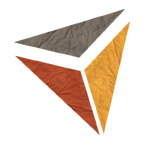
\includegraphics[width=\textwidth]{figures/i_demokratie}
        \caption{Demokratie}
        \label{fig:demo}
    \end{subfigure}
    \begin{subfigure}[t]{0.3\columnwidth}
        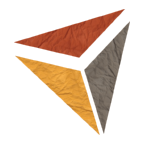
\includegraphics[width=\textwidth]{figures/i_macht}
        \caption{Macht}
        \label{fig:macht}
    \end{subfigure}
    \begin{subfigure}[t]{0.3\columnwidth}
        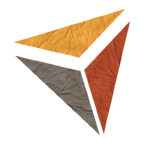
\includegraphics[width=\textwidth]{figures/i_partizipation}
        \caption{Partizipation}
        \label{fig:parti}
    \end{subfigure}
    \caption{Icon je nach Festival-Wochenende}
    \label{fig:icons}
\end{figure}

\begin{figure}[ht]
    \centering
        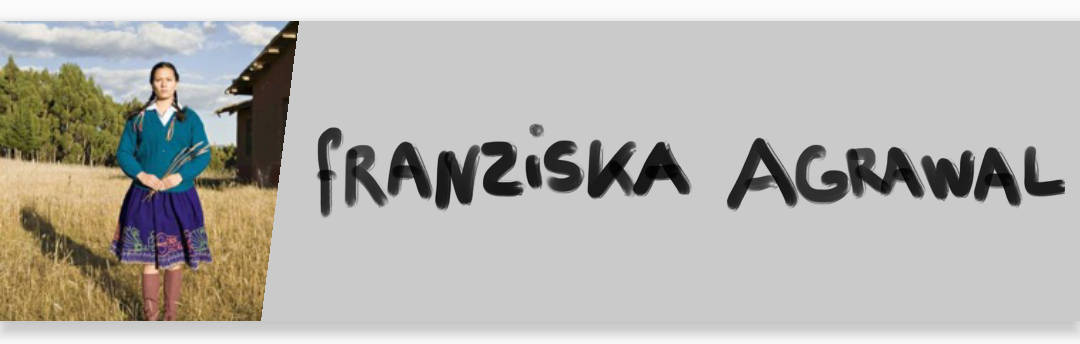
\includegraphics[width=.4\textwidth]{figures/kuenstler_item.png}
    \caption{Künstler mit abgeschnittenem Profilbild}
    \label{fig:kuenstler_item}
\end{figure}